\section{子问题一：电动汽车采用意愿分类}

\subsection{问题定义与难点}

任务一的目标是基于消费者画像与行为特征，预测ev\_adoption\_likelihood的Low、Medium、High三个等级。该任务的评分为准确率（权重20\%）。

核心难点包括：（1）\textbf{类别不均衡}——High类占比59.3\%，若全部预测为High先天准确率即达59.3\%；（2）\textbf{Medium的模糊性}——作为过渡等级，边界不清晰，相邻等级之间的误判是三分类模型的主要误差来源；（3）\textbf{特征与目标的关系非线性}——消费者采用意愿受收入、认知、态度、经济负担、出行需求等多因素交叉影响。

\subsection{探索性数据分析}

\subsubsection{目标变量分布}

如图\ref{fig:t1_target}所示，High类（59.3\%）约为Low类（16.5\%）的3.6倍，存在显著类别不均衡。

\begin{figure}[H]
\centering
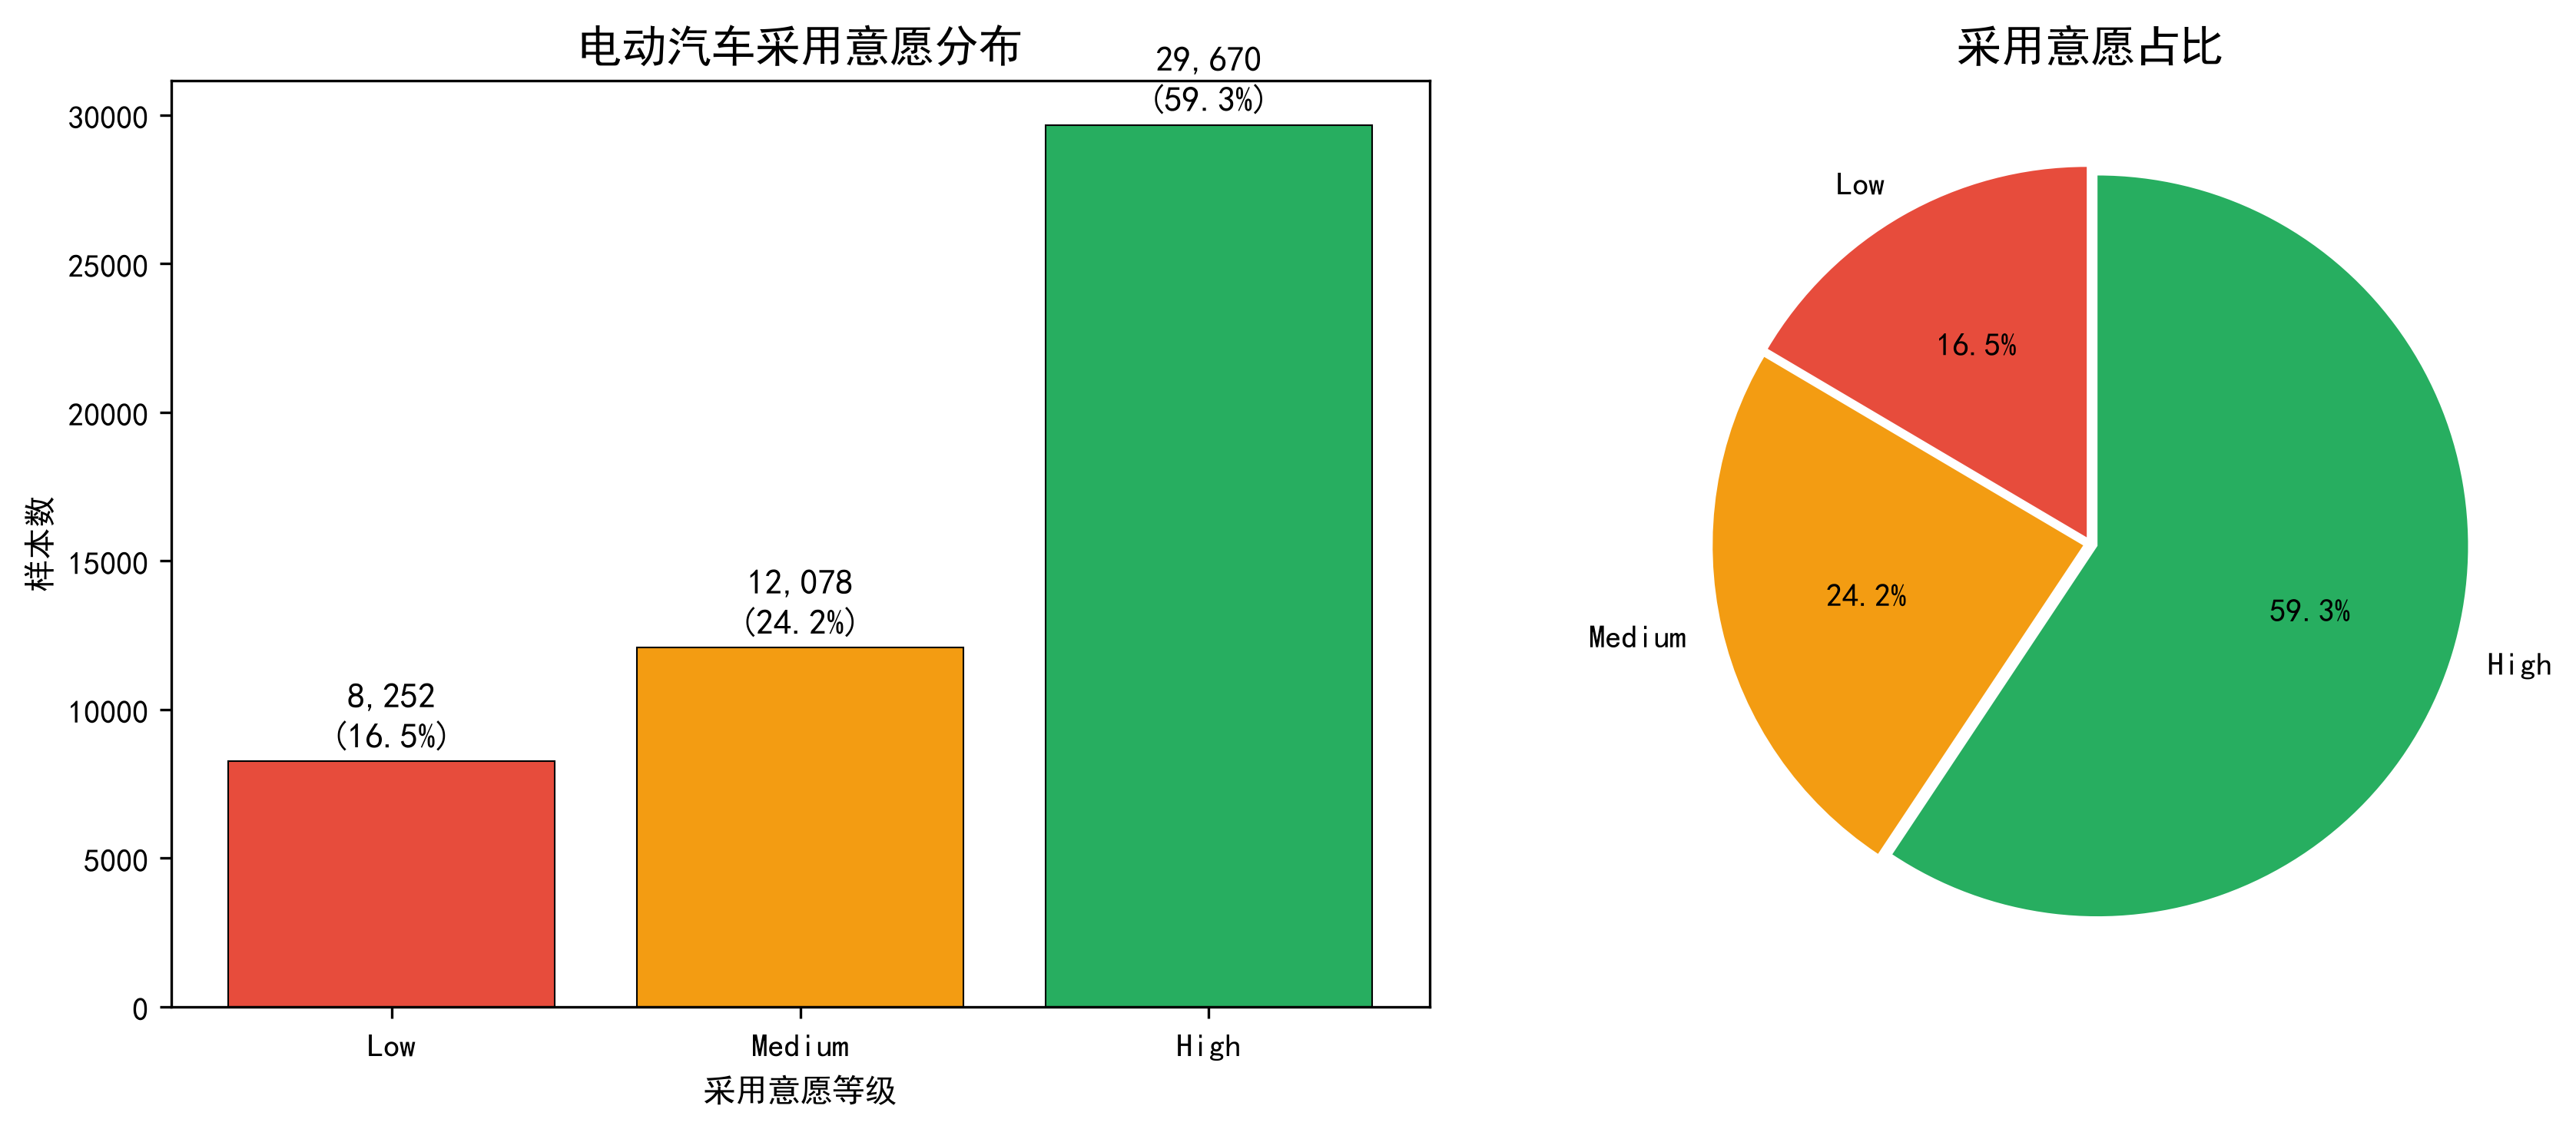
\includegraphics[width=0.9\textwidth]{figures/task1_target_distribution.png}
\caption{电动汽车采用意愿分布}
\label{fig:t1_target}
\end{figure}

\subsubsection{年收入与采用意愿的关系}

不同采用意愿群体的年收入分布如图\ref{fig:t1_income}所示。Low、Medium、High三组的中位数年收入分别约为2.6万、3.0万和4.7万美元，表明年收入是区分三类采用意愿的强因子。但三类之间存在较大重叠区域，仅靠收入阈值无法完美分离。

\begin{figure}[H]
\centering
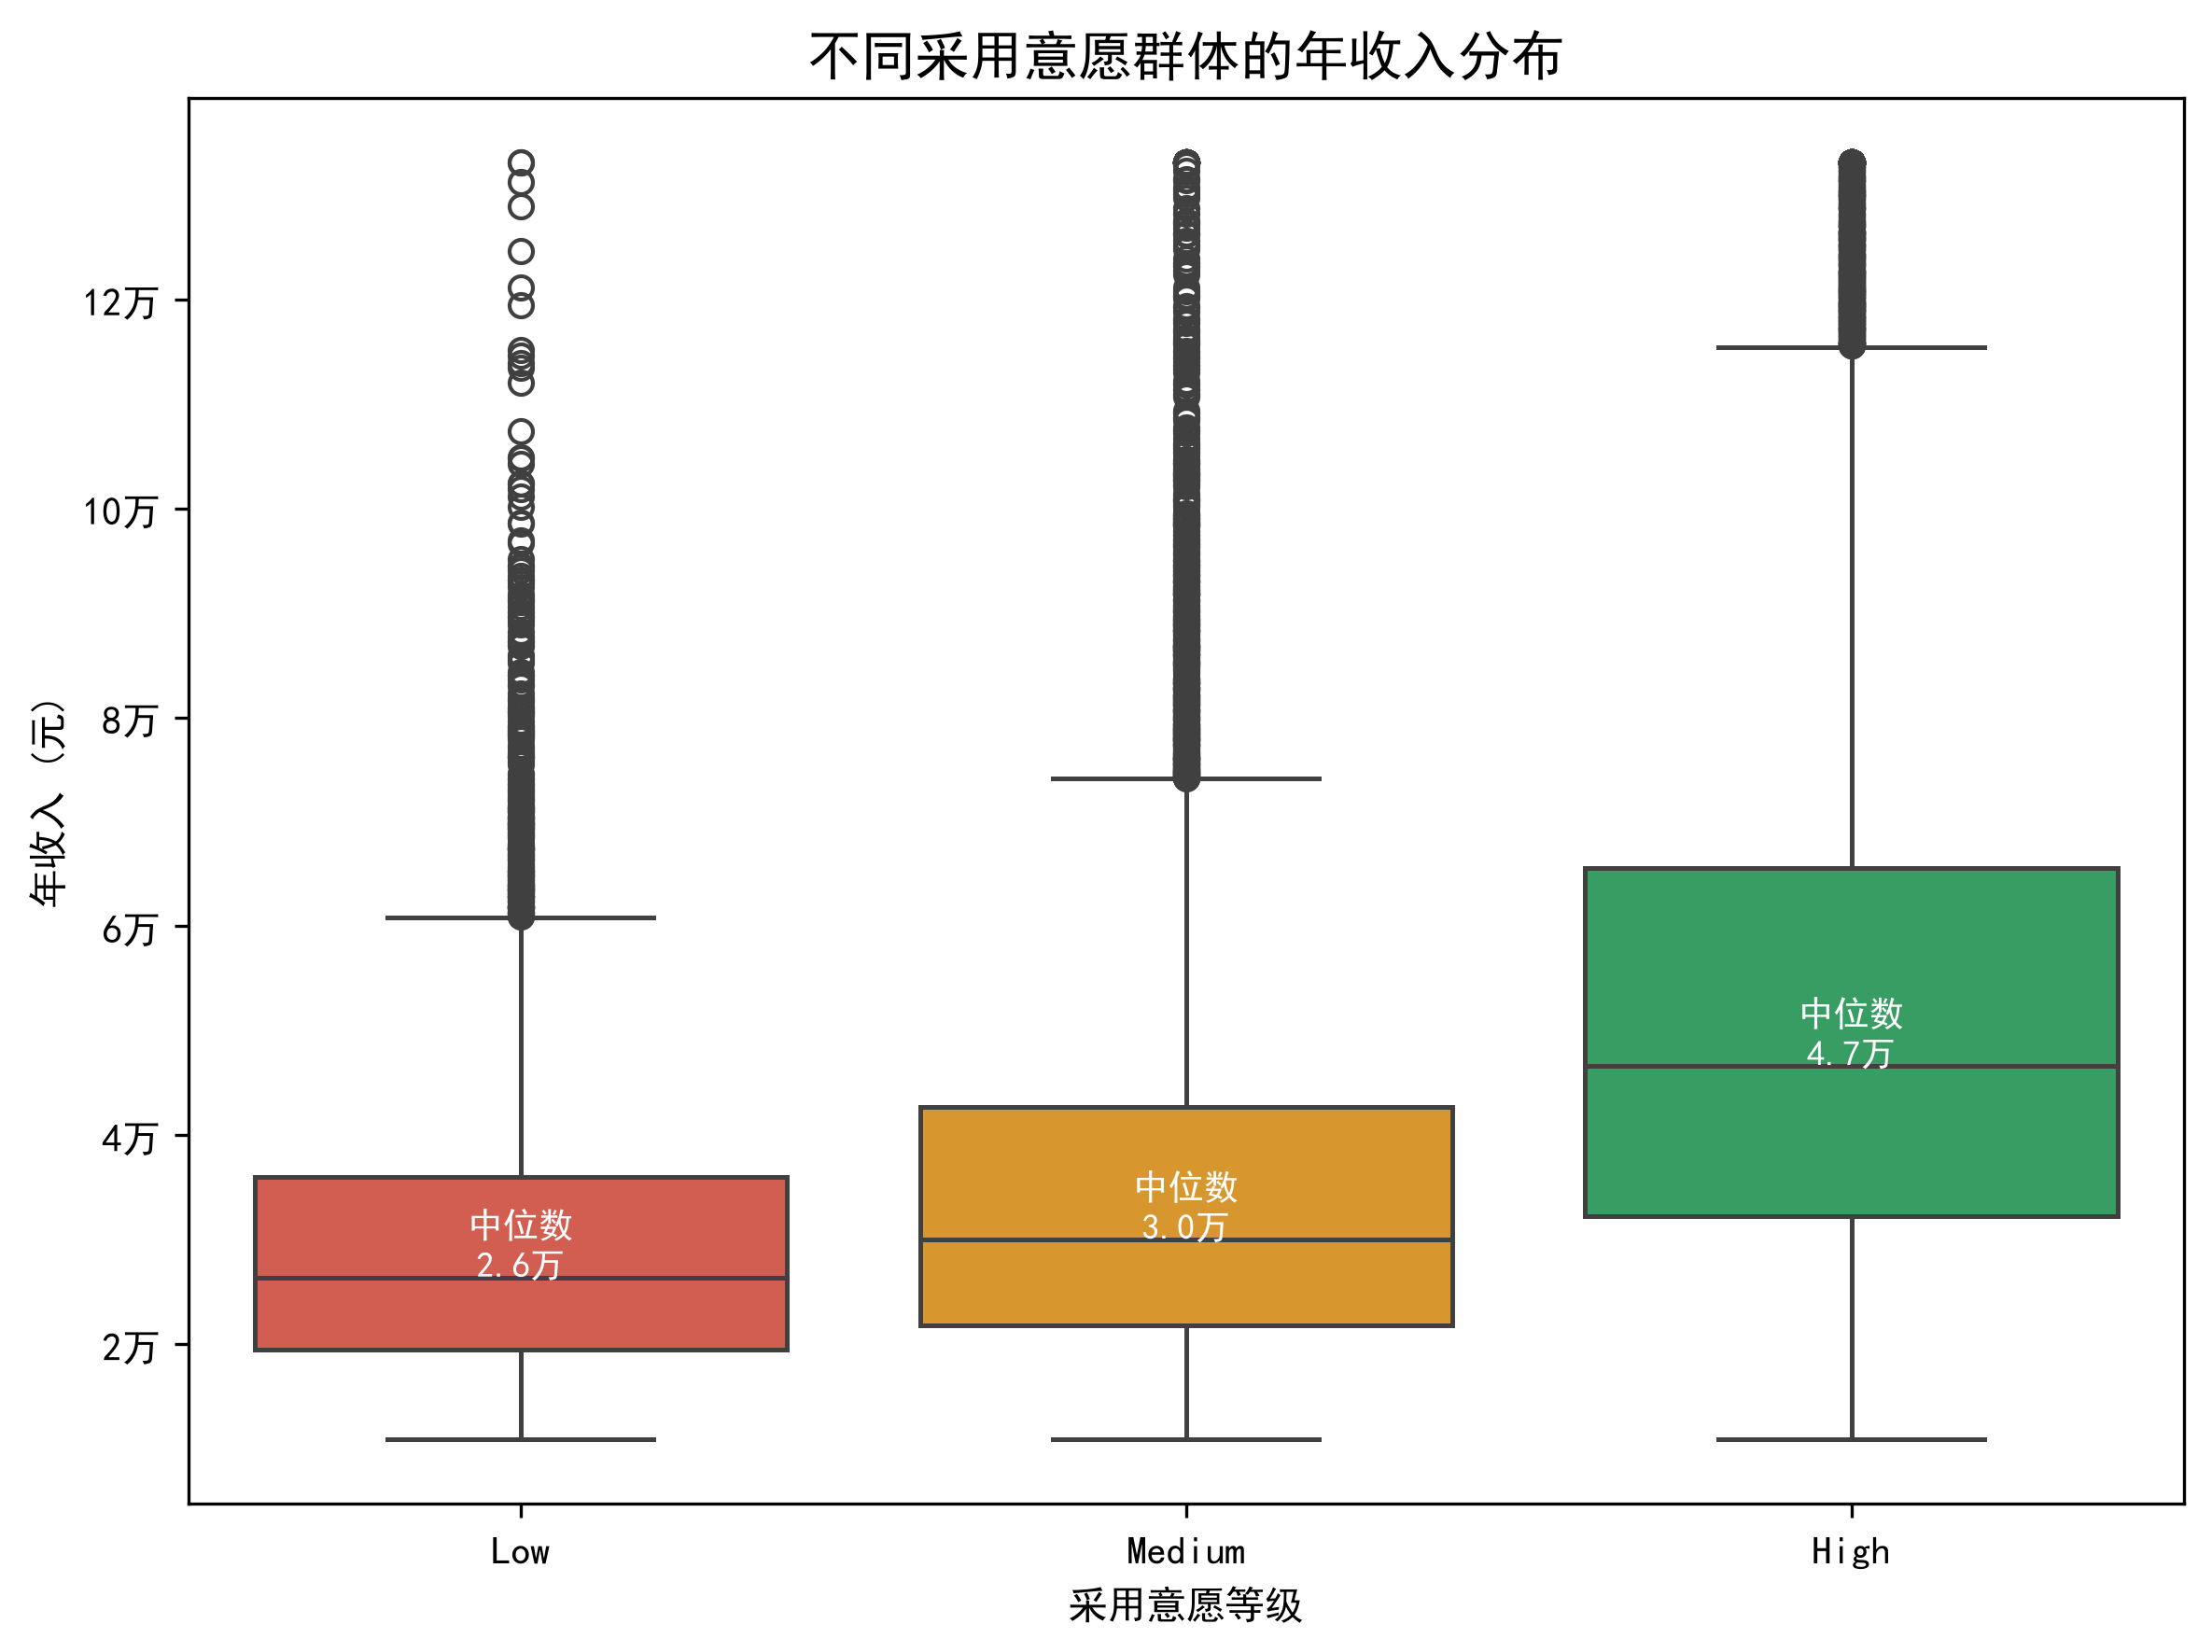
\includegraphics[width=0.8\textwidth]{figures/task1_income_boxplot.png}
\caption{不同采用意愿群体的年收入分布}
\label{fig:t1_income}
\end{figure}

\subsubsection{核心特征相关性分析}

热力图（图\ref{fig:t1_corr}）揭示了以下关键关系：
（1）daily\_commute\_km与weekly\_travel\_distance\_km相关系数为0.95，高度共线，直接同时入模可能导致信息冗余；
（2）range\_anxiety\_score与technology\_affinity\_score（-0.63）、ev\_knowledge\_score（-0.62）呈中高度负相关；
（3）environmental\_awareness\_score与ev\_knowledge\_score相关系数为0.75，表明环保意识与技术认知紧密关联。

\begin{figure}[H]
\centering
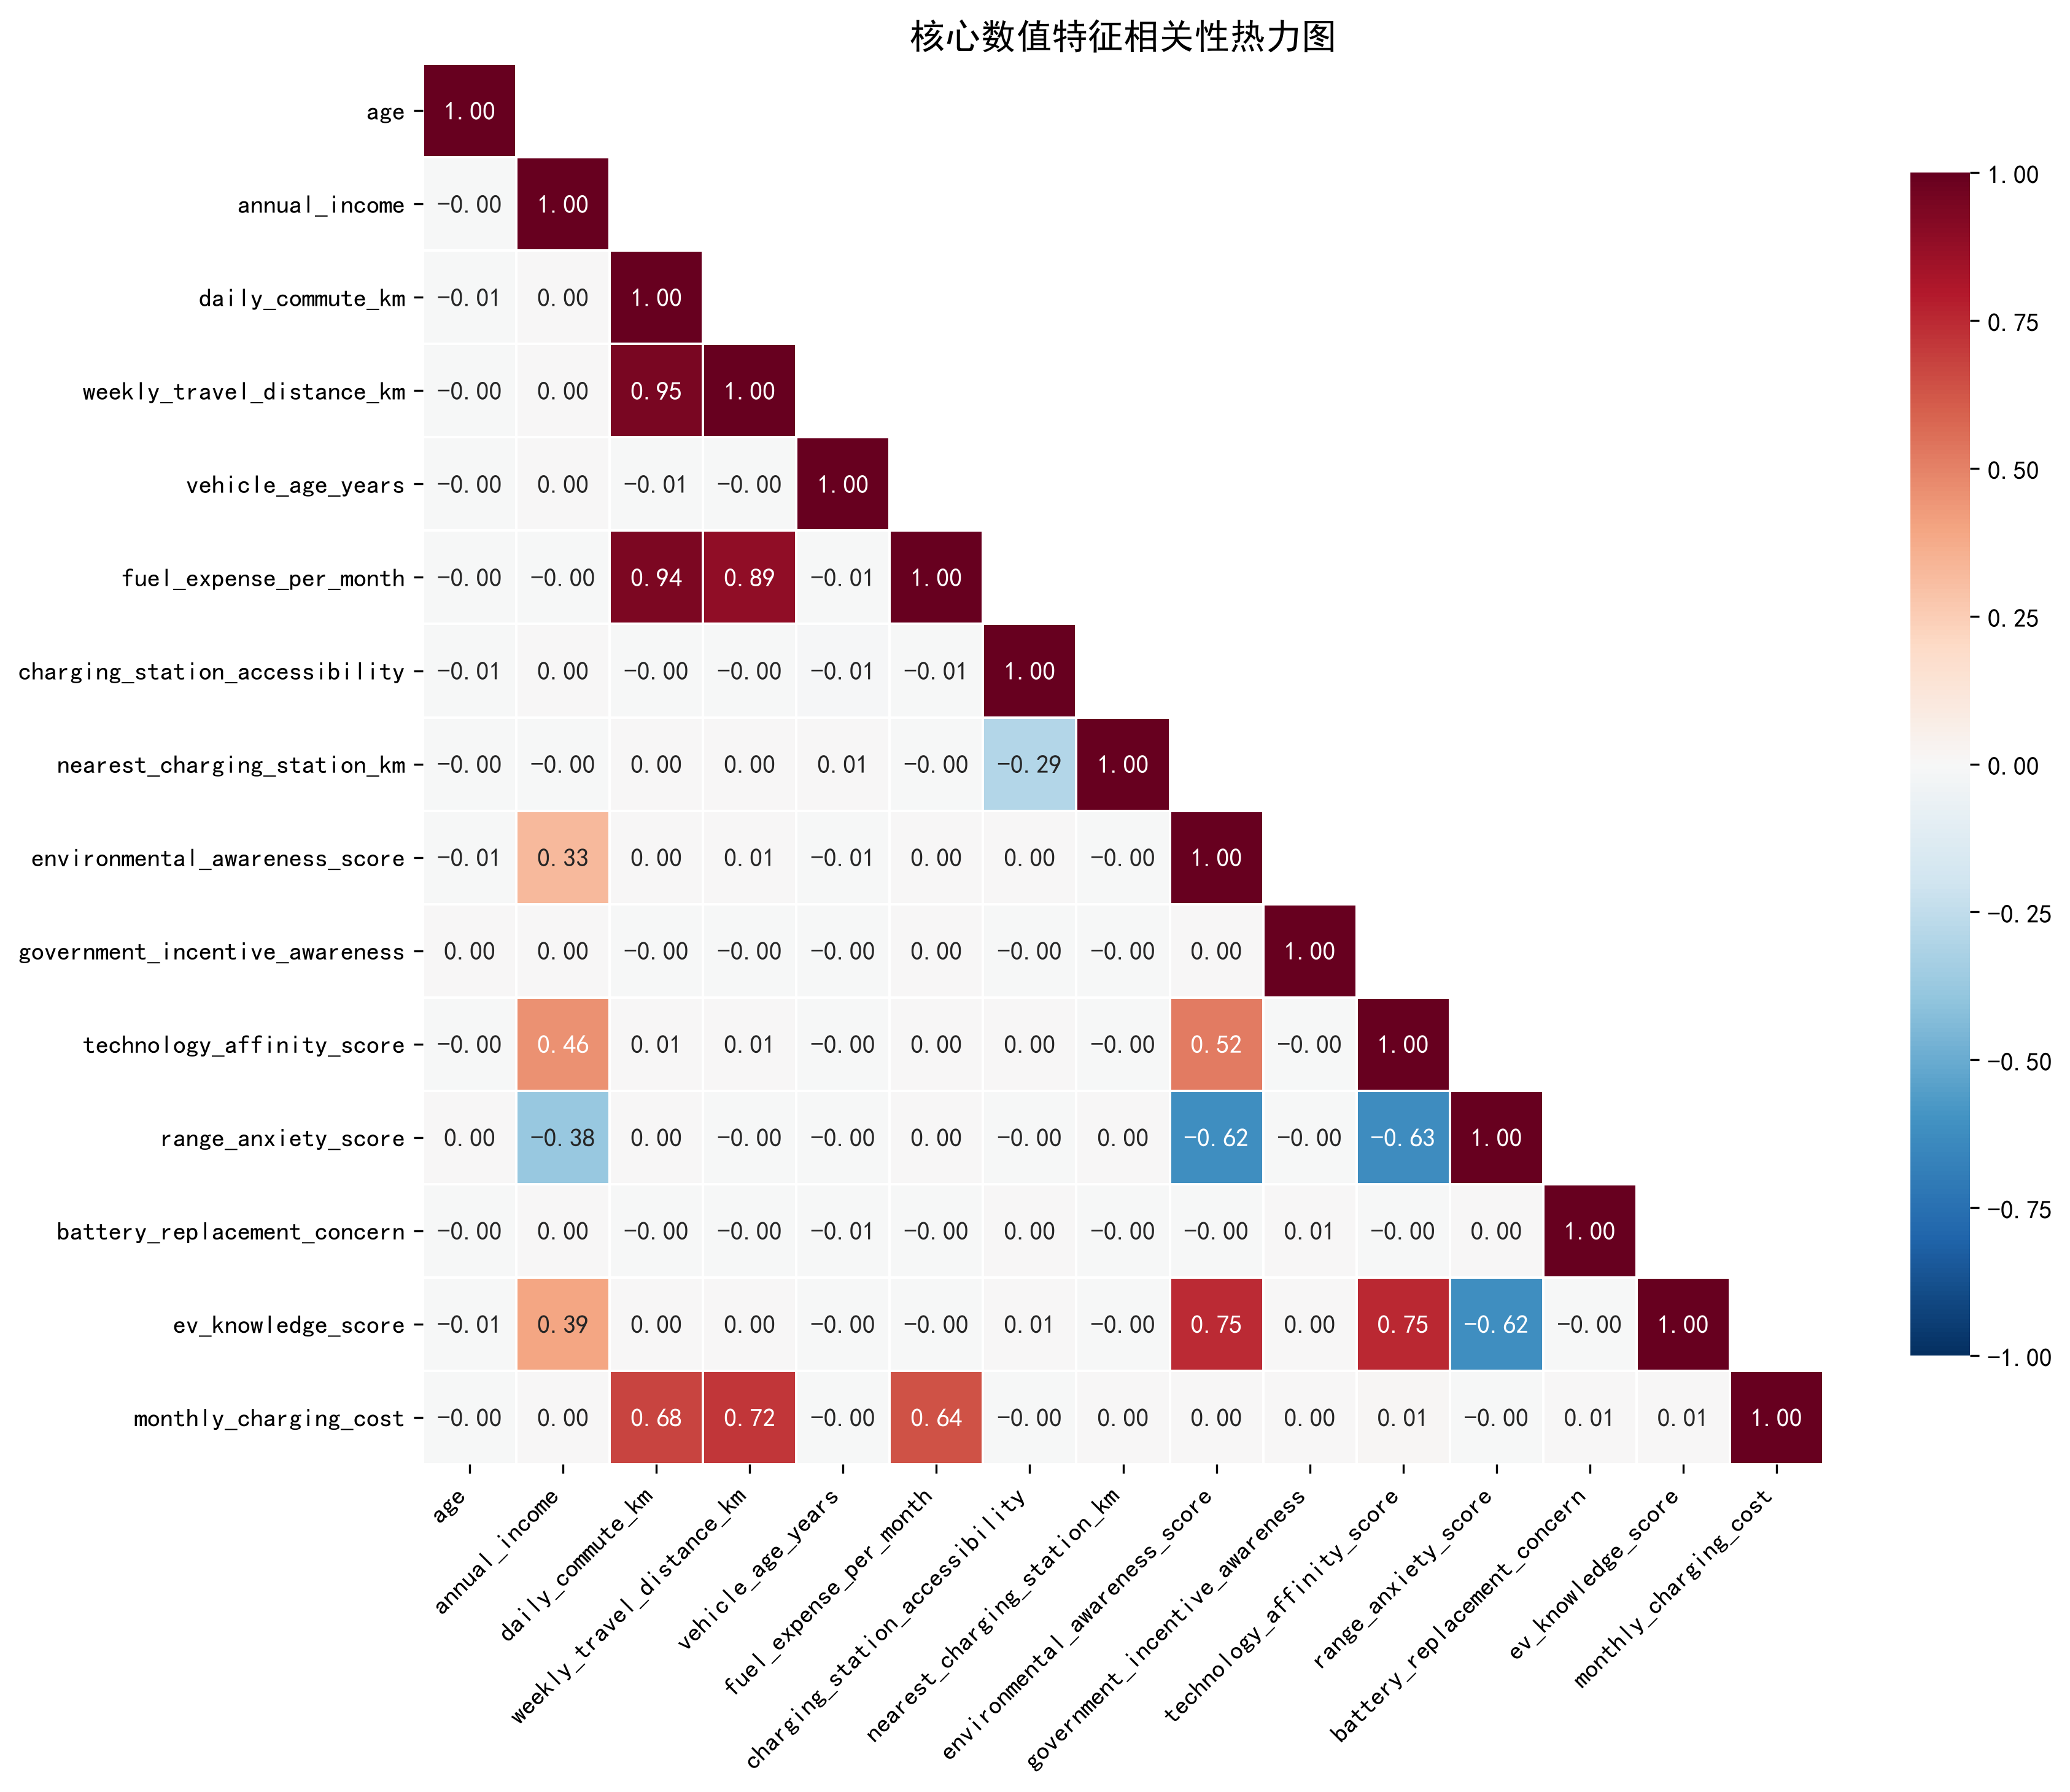
\includegraphics[width=0.85\textwidth]{figures/task1_correlation_heatmap.png}
\caption{核心数值特征相关性热力图}
\label{fig:t1_corr}
\end{figure}

\subsection{特征工程}

基于相关性分析和业务理解，针对任务一构造了8个业务交互特征，如表\ref{tab:t1_features}所示。

\begin{table}[H]
\centering
\caption{任务一业务交互特征}
\label{tab:t1_features}
\begin{tabular}{ccp{4.5cm}}
\toprule
\textbf{特征名称} & \textbf{计算公式} & \textbf{业务含义} \\
\midrule
fuel\_burden\_ratio & $\dfrac{12 \cdot \text{fuel\_expense}}{\text{annual\_income} + \varepsilon}$ & 燃油负担率：燃油成本对收入的压力 \\
travel\_consistency & $\dfrac{\text{weekly\_km}}{7 \cdot \text{daily\_km} + \varepsilon}$ & 出行一致性：$\approx$1为规律通勤，$>$1为不规律长途 \\
charging\_convenience & $\dfrac{\text{charging\_access}}{\text{nearest\_station} + 1}$ & 充电便利综合量：纳入主观可达性与客观距离 \\
green\_tech\_score & $\text{env\_aware} \times \text{tech\_aff}$ & 绿色技术倾向：两类态度的协同放大效应 \\
knowledge\_anxiety\_gap & $\text{ev\_know} - \text{range\_anxiety}$ & 认知焦虑差：EV知识能否抵消续航焦虑 \\
ev\_cost\_ratio & $\dfrac{12 \cdot \text{charge\_cost}}{\text{annual\_income} + \varepsilon}$ & 电动使用成本率：充电费用的经济压力 \\
replace\_tendency & $\text{veh\_age} \times \text{fuel\_expense}$ & 换车倾向近似：车龄与油耗的交互 \\
monthly\_disp\_income & $\text{annual\_income} / 12$ & 月可支配收入近似 \\
\bottomrule
\end{tabular}
\end{table}

注：$\varepsilon = 10^{-6}$防止除零，所有比值特征出现NaN时填0。

\subsection{训练策略与超参数}

采用三阶段递进式调参策略：
\begin{enumerate}[itemsep=0pt]
\item 第一轮（基线验证）：默认参数CatBoost + 原始特征，验证管线正确性；
\item 第二轮（特征消融）：对比原始特征/业务特征/类别权重方案；
\item 第三轮（超参数搜索）：随机搜索8组参数，5折分层CV下选择平均准确率最高的配置。
\end{enumerate}

CatBoost超参数搜索范围：depth $\in$ [5,9]，learning\_rate $\in$ [0.02,0.1]，iterations $\in$ [500,2000]，l2\_leaf\_reg $\in$ [3,15]，loss\_function=MultiClass，eval\_metric=Accuracy，early\_stopping\_rounds=200。类别权重消融测试了不加权、balanced和sqrt\_balanced三种方案。

\subsection{实验结果}

\subsubsection{验证集方案对比}

在10,000条独立验证集上，各方案的准确率对比如表\ref{tab:t1_results}所示。

\begin{table}[H]
\centering
\caption{任务一验证集方案对比}
\label{tab:t1_results}
\begin{tabular}{lcccc}
\toprule
\textbf{方案} & \textbf{ACC} & \textbf{Macro F1} & \textbf{Balanced ACC} & \textbf{说明} \\
\midrule
多数类基线 & $\approx$0.593 & -- & 0.333 & 全预测为High \\
LR 默认权重 & \textbf{0.8668} & 0.8294 & 0.8265 & 可解释性基线 \\
LR balanced权重 & 0.8575 & 0.8263 & 0.8400 & 加权提高少数类召回 \\
CatBoost 默认 (raw) & 0.8632 & 0.8251 & 0.8211 & 187轮早停 \\
CatBoost 默认 (+业务特征) & 0.8632 & 0.8245 & 0.8213 & 默认参数下未提升 \\
CatBoost 调参 (+业务特征) & 0.8633 & 0.8246 & 0.8213 & \textbf{最终模型} \\
\bottomrule
\end{tabular}
\end{table}

逻辑回归默认权重以0.8668的准确率略优于调参后CatBoost（0.8633），说明在40维特征空间中线性模型已能较好拟合。最终模型的最优参数为：depth=5，learning\_rate=0.05，iterations=1500，l2\_leaf\_reg=15，5折CV平均准确率为0.8730$\pm$0.0025。

\subsubsection{类别权重消融}

\begin{table}[H]
\centering
\caption{类别权重消融结果}
\label{tab:t1_weight}
\begin{tabular}{lc}
\toprule
\textbf{权重方案} & \textbf{5折CV准确率} \\
\midrule
不加权 & \textbf{0.8730} $\pm$ 0.0025 \\
balanced & 0.8713 $\pm$ 0.0018 \\
sqrt\_balanced & 0.8705 $\pm$ 0.0015 \\
\bottomrule
\end{tabular}
\end{table}

在竞赛以准确率为唯一指标的条件下，不加权方案最优。加权虽然提高了少数类召回，但牺牲了多数类预测准确率。

\subsubsection{混淆矩阵分析}

最终模型的验证集混淆矩阵如表\ref{tab:t1_conf}所示。

\begin{table}[H]
\centering
\caption{任务一混淆矩阵（验证集10,000样本）}
\label{tab:t1_conf}
\begin{tabular}{cccccc}
\toprule
\textbf{真实 $\backslash$ 预测} & \textbf{High} & \textbf{Low} & \textbf{Medium} & \textbf{样本数} & \textbf{误判率} \\
\midrule
High & 5,548 & 0 & 386 & 5,934 & 6.5\% \\
Low & 1 & 1,312 & 337 & 1,650 & 20.5\% \\
Medium & 397 & 246 & 1,773 & 2,416 & 26.6\% \\
\bottomrule
\end{tabular}
\end{table}

误判模式显示：（1）Low类误判主要流向Medium（99.7\%），仅1例被误解为High——模型能很好区分Low与High之间的鸿沟；（2）Medium类误判率最高（26.6\%），16.4\%被过判为High——作为过渡类别，同时受两端特征拖拽；（3）High类误判率仅6.5\%，零例流向Low，模型对多数类的识别非常自信。

\subsubsection{特征重要性排名}

CatBoost最终模型的PredictionValuesChange特征重要性Top 10如表\ref{tab:t1_import}所示。本研究构造的两个业务交互特征knowledge\_anxiety\_gap（得分21.68）和green\_tech\_score（得分20.03）占据前两位，远超出下一名battery\_replacement\_concern（9.68）。Top 10特征中6个属于认知与态度维度，说明采用意愿主要由心理认知因素驱动，经济因素起次要作用。

\begin{table}[H]
\centering
\caption{任务一特征重要性Top 10}
\label{tab:t1_import}
\begin{tabular}{clc}
\toprule
\textbf{排名} & \textbf{特征} & \textbf{重要性} \\
\midrule
1 & knowledge\_anxiety\_gap $\blacklozenge$ & 21.68 \\
2 & green\_tech\_score $\blacklozenge$ & 20.03 \\
3 & battery\_replacement\_concern & 9.68 \\
4 & charging\_station\_accessibility & 9.24 \\
5 & government\_incentive\_awareness & 7.64 \\
6 & charging\_convenience $\blacklozenge$ & 5.43 \\
7 & home\_charging\_available & 4.87 \\
8 & previous\_ev\_experience & 3.74 \\
9 & environmental\_awareness\_score & 2.22 \\
10 & range\_anxiety\_score & 1.98 \\
\bottomrule
\end{tabular}
\end{table}
注：$\blacklozenge$ 标记为本研究构造的业务交互特征。
